\documentclass[unicode, notheorems]{beamer}

% If you have more than three sections or more than three subsections in at least one section,
% you might want to use the [compress] switch. In this case, only the current (sub-) section
% is displayed in the header and not the full overview.
\mode<presentation>
{
  \usetheme[numbers, totalnumbers, minimal, compress]{Warsaw}

  \setbeamercovered{transparent}
  % or whatever (possibly just delete it)
}

%\usepackage{pscyr}
\usepackage[T2A]{fontenc}
\usepackage[utf8]{inputenc}
\usepackage[russian]{babel}
\usepackage{amsthm}

\usepackage{graphicx}
\graphicspath{ {media/} }


\usepackage{tikz}
\usetikzlibrary{arrows}
\usetikzlibrary{positioning}

% you only need this when using TikZ graphics

\newtheorem{theorem}{Теорема}
\newtheorem{example}{Пример}
\newtheorem{definition}{Определение}

\title{Имитационная модель американских опционов}

\author{Анастасия Миллер}
\institute[СПбГУ]{Санкт-Петербургский государственный университет \\
    Математико-механический факультет \\
    Кафедра статистического моделирования \\
    \vspace{0.4cm}
    Научный руководитель: д.ф.-м.н. Ермаков С.М. \\
    \vspace{0.3cm}
}
\date{
    Санкт-Петербург\\
    \today
}

% \subject{Beamer}
% This is only inserted into the PDF information catalog. Can be left
% out.

% Delete this, if you do not want the table of contents to pop up at
% the beginning of each subsection:
% \AtBeginSubsection[]
% {
%   \begin{frame}<beamer>
%     \frametitle{Outline}
%     \tableofcontents[currentsection,currentsubsection]
%   \end{frame}
% }

\begin{document}

\begin{frame}
    \titlepage
\end{frame}

\section{Постановка задачи}

  \begin{frame}
    \frametitle{Основные понятия}

    \begin{definition}
      \emph{Опцион} -- договор, по которому потенциальный покупатель или потенциальный продавец актива (товара, ценной бумаги) получает право, но не обязательство, совершить покупку или продажу данного актива по заранее оговорённой цене в определённый договором момент в будущем или на протяжении определённого отрезка времени.
    \end{definition}
  \end{frame}

  \begin{frame}
    \frametitle{Основные понятия}
% Задача -- частный случай более общей проблемы оптимального времени остановки. Имеет аналитическое решение в случае бесконечного горизонта (неограниченной валидности опциона) (Karatzas, Ioannis; Shreve, Steven E. (1998). "Methods of Mathematical Finance". Stochastic Modelling and Applied Probability 39), аналитическое решение в случае конечного горизонта неизвестно (http://en.wikipedia.org/wiki/Optimal_stopping#Option_trading).
    \begin{block}{}
    Справедливой ценой опциона будет максимальная выручка, которую можно получить от исполнения опциона:
    $$\max_{\tau\in \left[0;T\right]}E\left( e^{-rt} \left( S_\tau - K \right)^+ \right)$$\footnotemark
    \end{block}
    Дискретные оценки: состояние актива меняется только в определённых точках $t_0,\ldots,t_n \in \left[0;T\right], n < \infty$.
    \footnotetext[1]{$S_\tau$ в зависимости от контекста обозначает либо состояние базового актива, либо цену, которую можно получить за него на рынке}
  \end{frame}

  \begin{frame}
    \frametitle{Основные понятия}
    Дискретизация процесса даёт оценку
    $$\left\lbrace \begin{aligned}
        V_i(X_i) &= \max \left\lbrace e^{-rt_i} \left( S_{t_i} - K \right)^+, EV_{i+1}(X_{i+1}) \right\rbrace, i\in 1:n-1 \\
        V_n(X_n) &= e^{-rt_n} \left( S_{t_n} - K \right)^+
    \end{aligned}\right.$$
    здесь $V_0(X_0)$ --- цена опциона, исполняемого $n$ раз в году, на момент выписывания которого базовый актив был в состоянии $X_0$
  \end{frame}

\section{Случайные деревья}
    \begin{frame}
        \frametitle{Случайные траектории}
        Будем оценивать $V_0(S_0)$ методом Монте-Карло.
        \visible<2->
        \\ Промоделируем много вариантов жизни базового актива. Траектория --- набор состояний $S_{t_1}, \ldots, S_{t_n}$.
        \begin{figure}[h]
            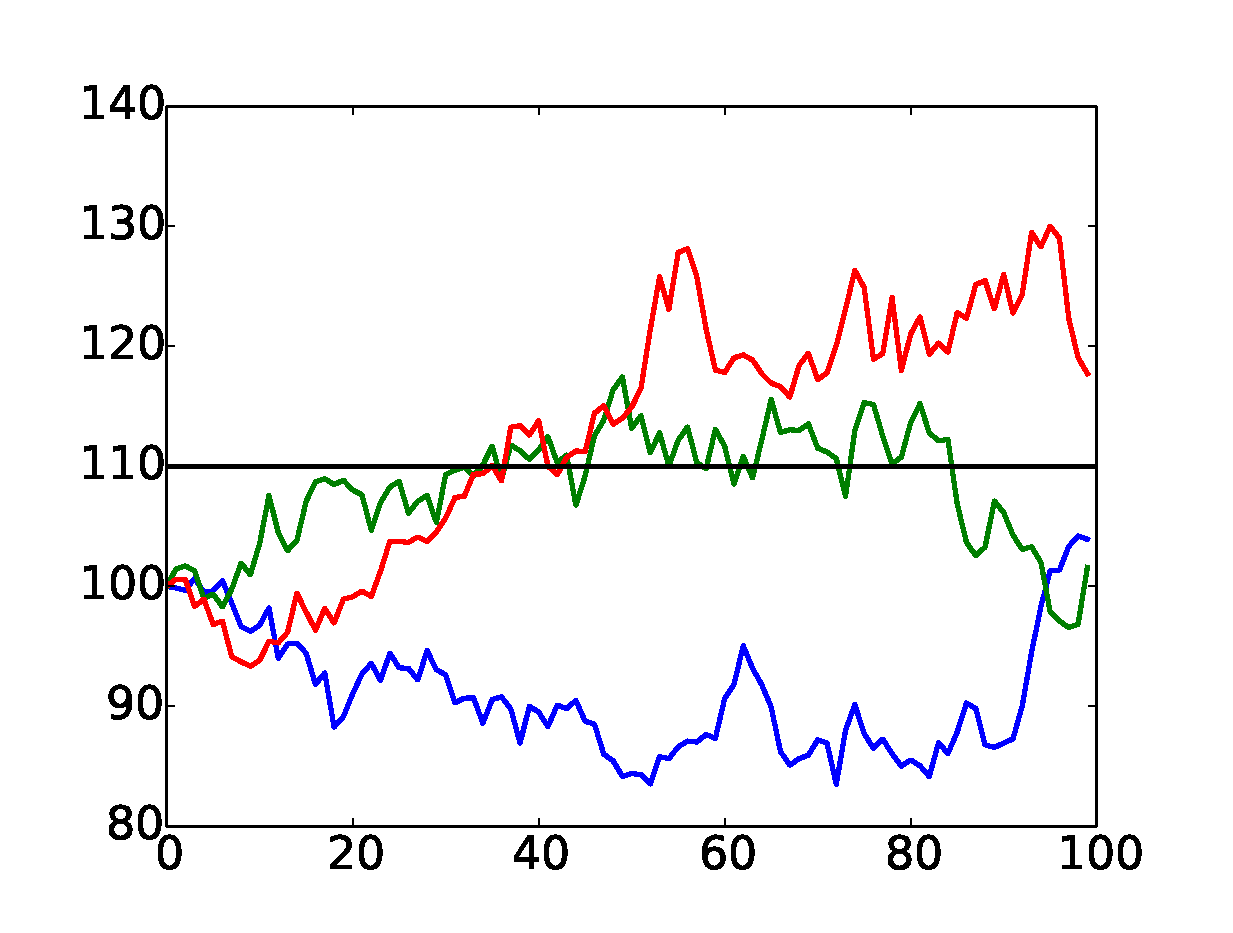
\includegraphics[height=0.4\paperheight]{traces}
            \caption{Возможные траектории цены базового актива, горизонтальная линия -- цена страйк}
            \label{fig:traces}
        \end{figure}
    \end{frame}

\begin{frame}
    \frametitle{Случайные деревья}
    Дерево -- способ получить больше траекторий в том же объёме памяти. Построение дерева:
    \begin{figure}[h]
        картинка про дерево
    \end{figure}
\end{frame}

\begin{frame}
    \frametitle{Случайные деревья}
    Число вершин в дереве -- $$\sum_{k=0}^n b^k = \frac{b^{n+1} - 1}{b-1} = O(b^n)$$
    Число вершин уменьшится, если считать достаточно близкие вершини одинаковыми
\end{frame}

\begin{frame}
    \frametitle{Квантили эмпирического распределения}
    $S_i^j, i \in 1:b, j\in 1:k$ --- все промоделированные состояния базового актива, относящиеся к одному времени.
    $$F_{S_i^j}(x) = \frac{1}{bk}\#\left\lbrace (i, j) \in 1:b \times 1:k \middle\vert S_i^j < x \right\rbrace$$
    Группировка по квантилям:
    $$A_j = \left\lbrace S_i^j \middle\vert \frac{j-1}{n} < F_{S_\tau}\left( S_i^j\right) < \frac{j}{n}\right\rbrace$$
    Все вершины, принадлежащие множеству $A_j$, заменяются на $\mathsf{med}A_j$.
\end{frame}

\begin{frame}
    \frametitle{Случайные деревья}
    \begin{figure}
    \centering
    \begin{tikzpicture}[->,>=stealth',shorten >=1pt,auto,node distance=0.35\linewidth, main node/.style={rectangle,draw}]

        \node[main node] (2) {97}
            child { node[main node] (88) {88}}
            child { node[main node] (92) {92}}
            child { node[main node] (106) {106}};
        \node[main node] (3) [right of=2] {103}
            child { node[main node] (96) {96}}
            child { node[main node] (115) {115}}
            child { node[main node] (107) {107}};
        \node[main node] (1) [right of=3] {110}
            child { node[main node] (116) {116}}
            child { node[main node] (104) {104}}
            child { node[main node] (112) {112}};

        \node[main node] (92s) [below=0.1\paperheight of 92]{92}
            child { node[main node] (92r) {92}};
        \path (92) edge[<->] (92s);
        \node[main node] (88s) [below=0.1\paperheight of 88] {88};
        \path (88) edge[<->] (88s)
            (88s) edge (92r);
        \node[main node] (96s) [below=0.1\paperheight of 106]{96};
        \path (96) edge[<->] (96s)
            (96s) edge (92r);

        \node[main node] (106s) [below=0.1\paperheight of 115]{106}
            child { node[main node] (106r) {106}};
        \path (106) edge[<->] (106s);
        \node[main node] (104s) [below=0.1\paperheight of 96]{104};
        \path (104) edge[<->] (104s)
            (104s) edge (106r);
        \node[main node] (107s) [below=0.1\paperheight of 107]{107};
        \path (107) edge[<->] (107s)
            (107s) edge (106r);

        \node[main node] (115s) [below=0.1\paperheight of 104]{115}
            child { node[main node] (115r) {115}};
        \path (115) edge[<->] (115s);
        \node[main node] (112s) [below=0.1\paperheight of 116]{112};
        \path (112) edge[<->] (112s)
            (112s) edge (115r);
        \node[main node] (116s) [below=0.1\paperheight of 112]{116};
        \path (116) edge[<->] (116s)
            (116s) edge (115r);

    \end{tikzpicture}
    \caption{Пример прореживания дерева}
    \label{fig:reduceTree}
    \end{figure}

\end{frame}

\begin{frame}\frametitle{Оценки $V_0(X_0)$по прореженному и точному дереву}
    \begin{columns}
        \begin{column}{0.5\textwidth}
            \begin{figure}
                \centering
                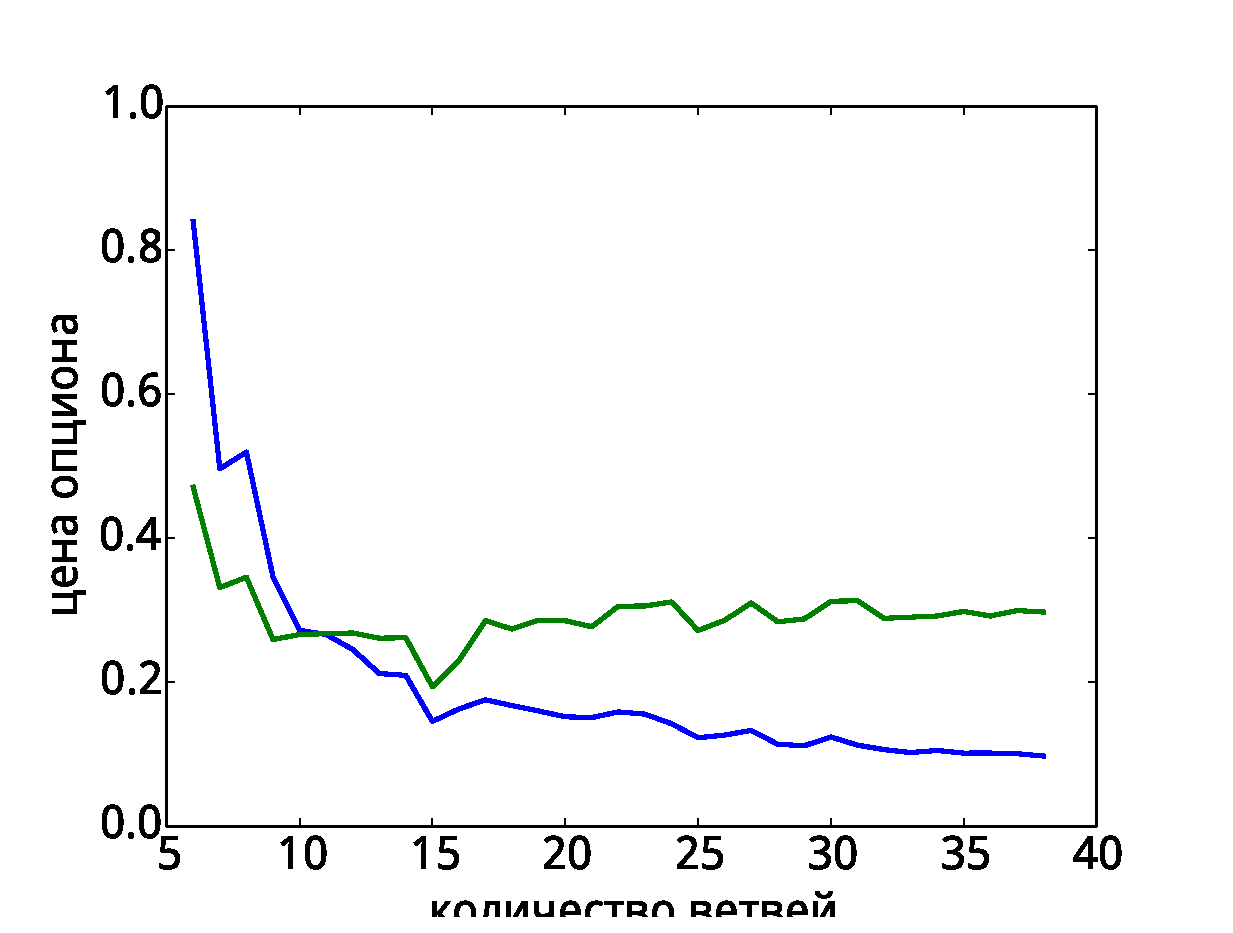
\includegraphics[width=\linewidth]{true_value_test_empiric_distr}
                \caption{Прореженное дерево}
                \label{fig:true_value_test_empiric_distrib}
            \end{figure}
        \end{column}
        \begin{column}{0.5\textwidth}
            \begin{figure}
                \centering
                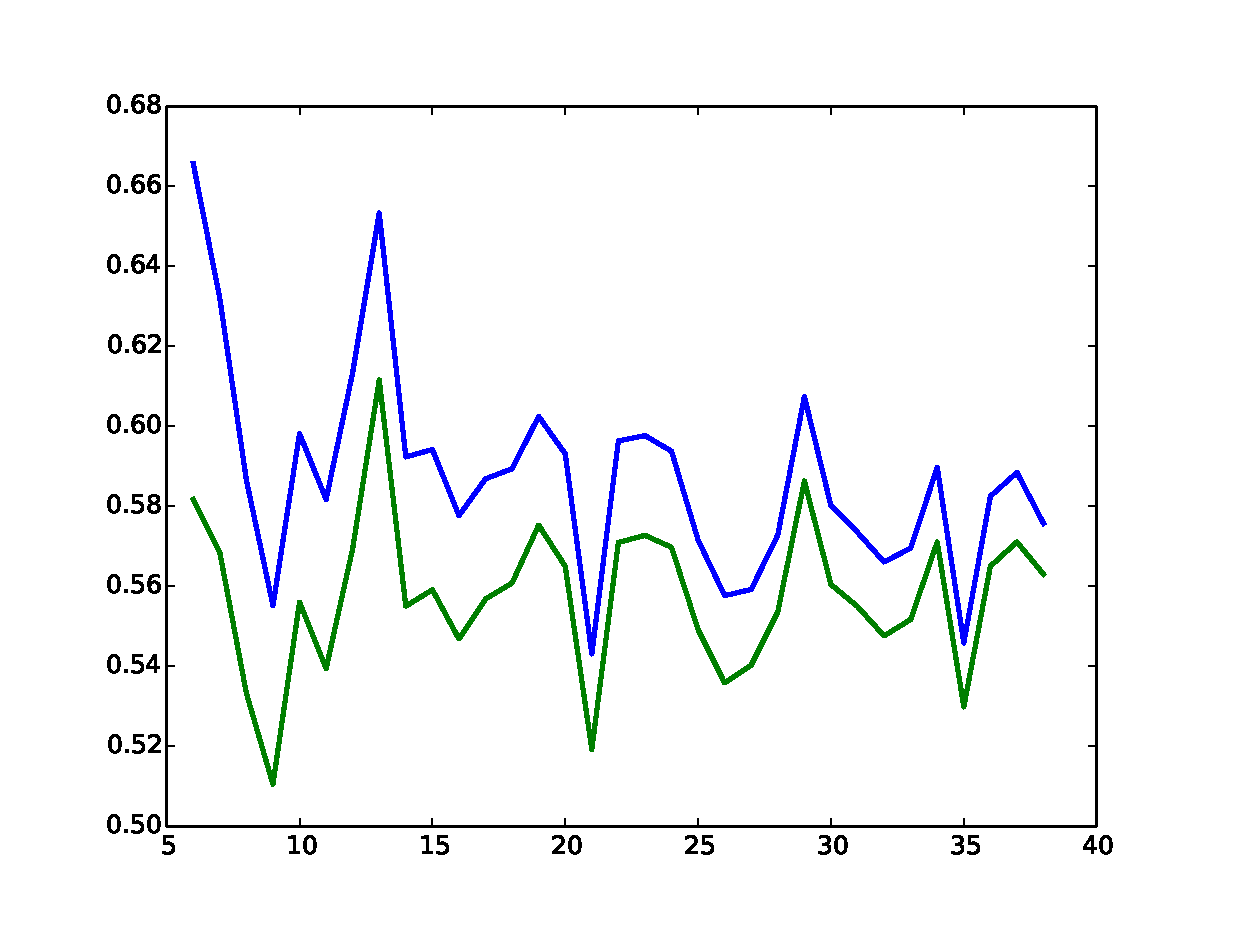
\includegraphics[width=\linewidth]{true_value_test_standard}
                \caption{Обычное дерево}
                \label{fig:true_value_test_standard}
            \end{figure}
    \end{column}
\end{columns}
\end{frame}



  \begin{frame}
    \frametitle{Планы}
    \begin{enumerate}
    \item Закончить рассмотрение оценки по гистограмме, в т.ч.\ найти аналитически математическое ожидание оценки
    \item Рассмотреть оценку по кластерам
    \item Рассмотреть другие оценки
  \end{enumerate}
  \end{frame}

\end{document}
